
According to the specification, the first objective in the development of the project is to design a an FPGA module that directly connects the audio inputs to the outputs. Therefore, the work done so far has mostly consisted in \textit{research} on audio data transmission and \textit{attempts} of recreating a stable input-output system.

\subsection{Audio Inputs and Outputs on the Zybo Board}

The target device for this project (Digilent Zybo Z7 board) contains three analogue 3.5mm standard jack ports (Microphone In, Line In and Headphone Out). The analogue signals received through these connections are converted using the board's integrated ADC (analogue-to-digital converter). Therefore, from the perspective of the FPGA designer, the inputs can only be seen as 1-bit digital signals.

% \subsubsection{I2S Protocol}

The Zybo Z7 board is using the \textbf{I2S (Inter-IC Sound)}\cite{i2s} protocol to transfer the audio data, a serial link designed especially for transmitting digital audio data, which was introduced in 1986 by Philips Semiconductor.

\begin{figure}[h]
    \centering
    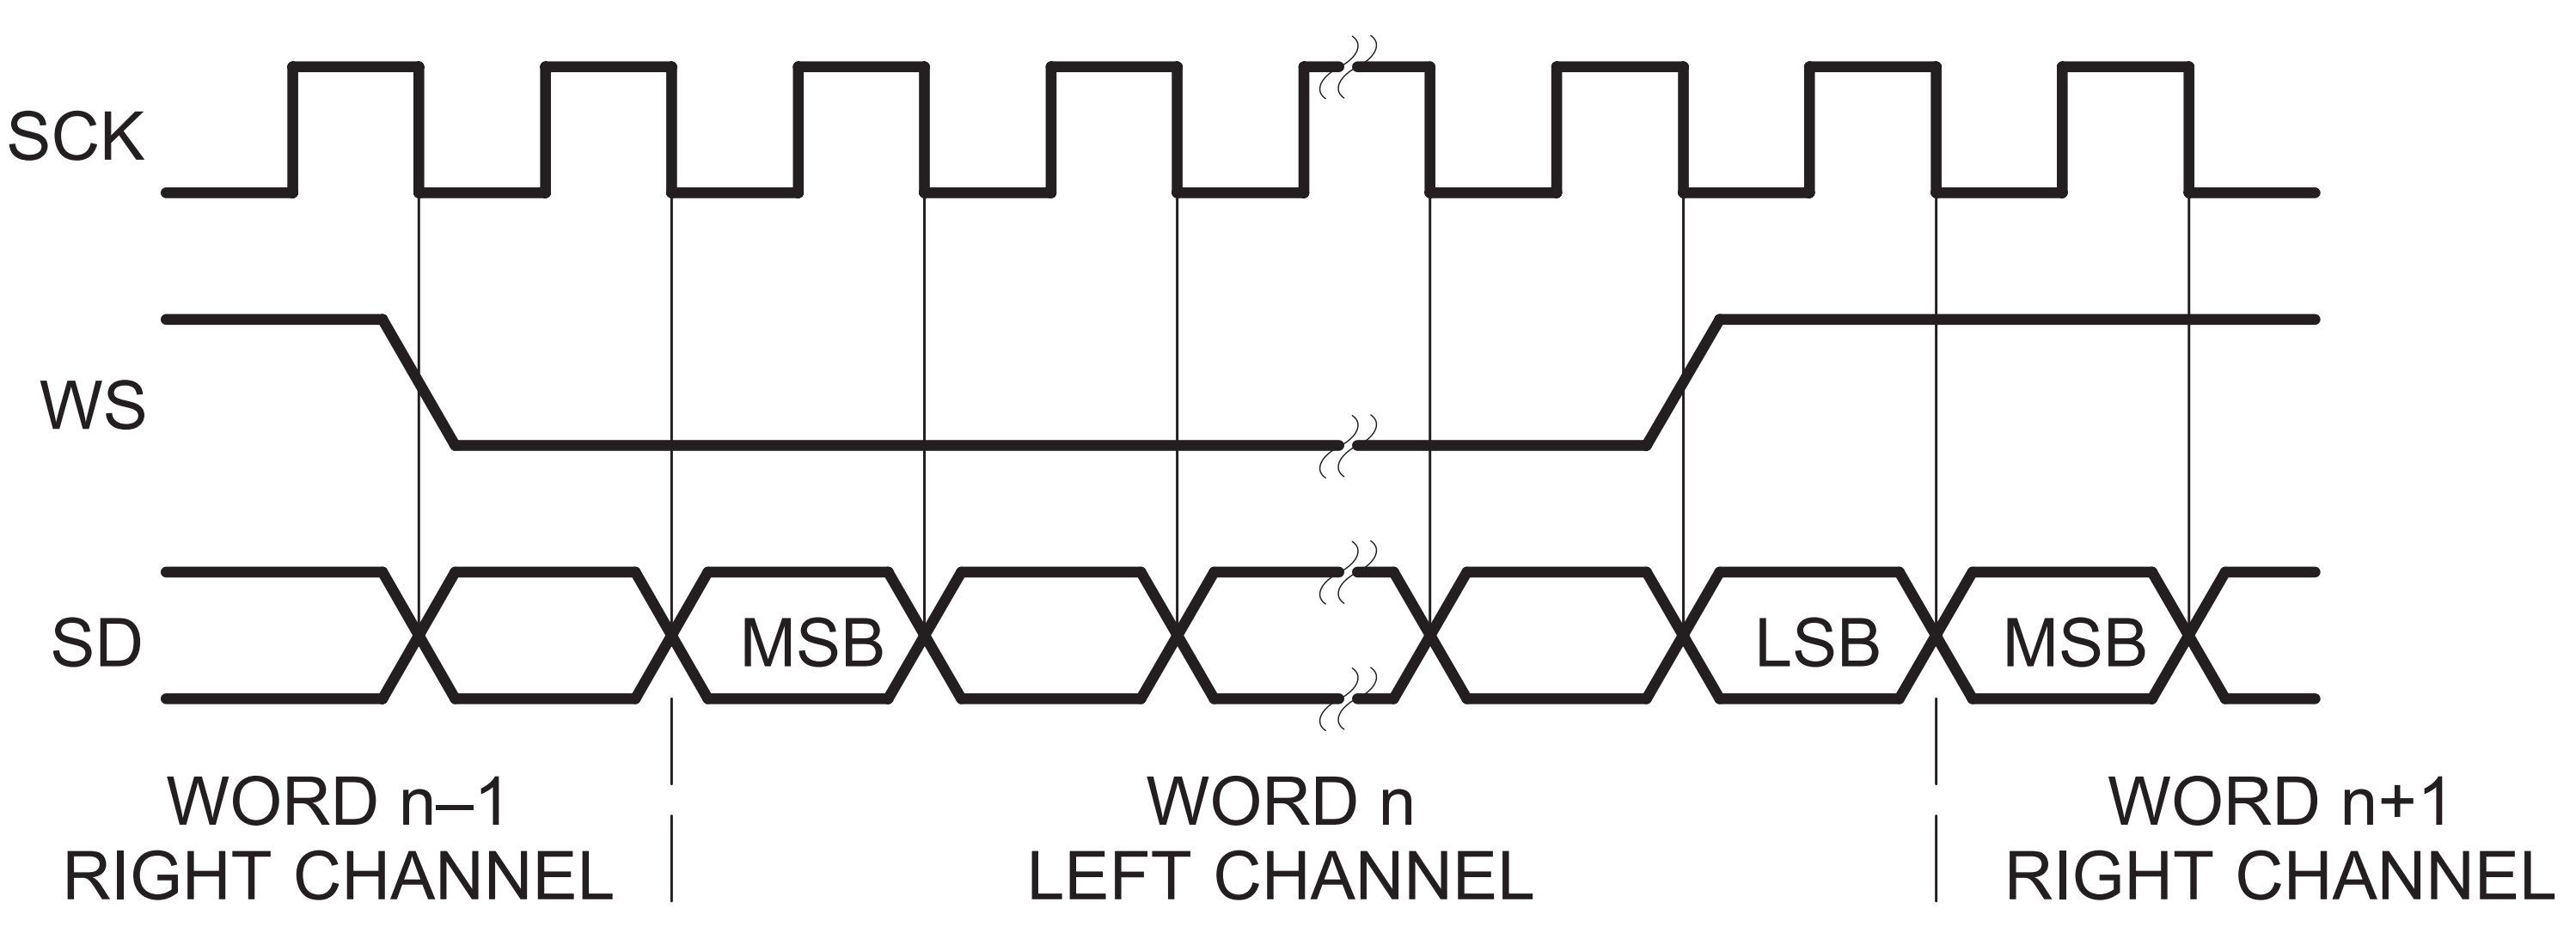
\includegraphics[width=0.9\linewidth]{progress-report/i2s-timing.png}
    \caption{I2S Basic Interface Timing}
    \label{fig:i2s-timing}
\end{figure}


As shown in Figure \ref{fig:i2s-timing}, the bus has three lines (each of 1-bit width). The signals are described in Table \ref{tab:i2s-signal-descriptions}.

\begin{table}[h]
    \centering
    \begin{tabular}{|p{1.3cm}|p{2cm}|p{12cm}|}
        \hline
        \textbf{Symbol} & \textbf{Name} & \textbf{Description} \\
        \hline
        SCK & Continuous Serial Clock & A clock generated by the controller device, that determines the data transmission rate.\\
        \hline
        SD & Serial Data & Audio data transmitted in two's complement. \\
        \hline
        WS & Word select & The word select line indicates the channel being transmitted (WS = 0 for left channel, and WS = 1 for right channel).\\
        & & - The WS signal changes one clock cycle after the MSB is transmitted, which allows a clock cycle for other necessary calculations.\\
        & & - The WS is also generated by the controller device\\
        \hline
    \end{tabular}
    \caption{I2S Signal Descriptions}
    \label{tab:i2s-signal-descriptions}
\end{table}

\subsubsection{Using the Audio Data}

The audio pins available for controlling the Audio Codec on the Zybo board are listed in Table \ref{tab:Zybo-AC-signals}. Based on the reference manual\cite{zybo-ref-man} from the board manufacturer, an investigation was conducted on how these signals must be interpreted and configured.

\begin{table}
    \centering
    \begin{tabular}{|p{1.5cm}|p{1.5cm}|p{12cm}|}
        \hline
        \textbf{Signal name} & \textbf{Direction} & \textbf{Description and Desired Configuration} \\
        \hline
        MCLK & output & The Master Clock must be an integer multiple of the desired sampling rate. For default settings, a master clock of 12.288 MHz is used, resulting in a 48 kHz sampling rate. \\
        \hline
        MUTE & output & The Mute signal is an active-low signal that disables the analogue outputs. Therefore, it must be set to high. \\
        \hline
        BCLK & output & This signal is the serial clock used by the I2S. It defines the rate at which our data is collected from the ADC. The frame is 32 bits per sample, and there are two samples per frame, meaning there are 64 clocks needed to transfer a frame. Therefore, BCLK is always 64 times LRCLK. With a sampling frequency of 48 kHz, BCLK must be 3.072 MHz. We are using 256x oversampling (the MCLK is set at fs * 256), the BCLK can be obtained by dividing the MCLK by 4. \\
        \hline
        PBLRC and \mbox{RECLRC} & output & The PBLRC and RECLRC signals determine whether the data received/transmitted on the data ports (PBDAT/RECDAT) corresponds to the left or right audio channel. Since the input and output data ports have the same sampling rate and the same number of channels, the signals can be joined together as a clock of frequency 48 kHz. \\
        \hline
        RECDAT & input & This 1-bit wide signal transmits the actual data received from the Mic/Line-in analogue port. The data starts from the MSB, and it is transmitted on the negative edge of the BCLK. The data is sent 1 clock cycle after the LRCLK has changed. \\
        \hline
        PBDAT & output & This 1-bit wide signal transmits the actual data sent to the Headphone analogue port. The data starts from the MSB, and it is transmitted on the negative edge of the BCLK. The data is sent 1 clock cycle after the LRCLK has changed. \\
        \hline
        SCL & output & Unused signal \\
        \hline
        SDA & input or output & Unused signal \\
        \hline
    \end{tabular}
    \caption{Zybo Z7 Audio Codec Signal Descriptions and Configurations}
    \label{tab:Zybo-AC-signals}
\end{table}

The last two signals presented in the table are used for configuring the format of the Audio Codec (AC), and can be interpreted using the I2C (Inter Integrated Circuit)\cite{i2c} protocol. For the scope of this project, the AC is used with default settings, and these signal do not need to be driven.

% \subsubsection{Using the Audio Data}

All the signals received and transmitted through the pins have a 1-bit width, meaning no straightforward calculations can be performed on the data in this format. Therefore, the next objective is to convert the data into registers.

A very important resource for this is the ``Zybo Z7 DMA Audio Demo''\cite{dma-demo}, tutorial, as it demonstrates the configuration of the Audio Codec for both receiving and transmitting data on the board's jack inputs. A crucial feature of the demo is the implementation of \textbf{FIFO modules} on both input and output registers. This component allows performing operations on data sampled at different points in time, and must be recreated int the audio processor.

\subsection{Current Situation}
The current status of the project consists in a working input-output system, with data stored as registers. However, development is still ongoing for introducing the FIFO modules and deciding on their configuration.

Nevertheless, the accuracy of the design decisions is not the main focus at this point in the project. The design consists of many moving parts, which are subject to change as soon as the development of the audio effects begins. A simplified diagram of the desired product can be found in Figure \ref{fig:system-diagram}.

\begin{figure}[h]
    \centering
    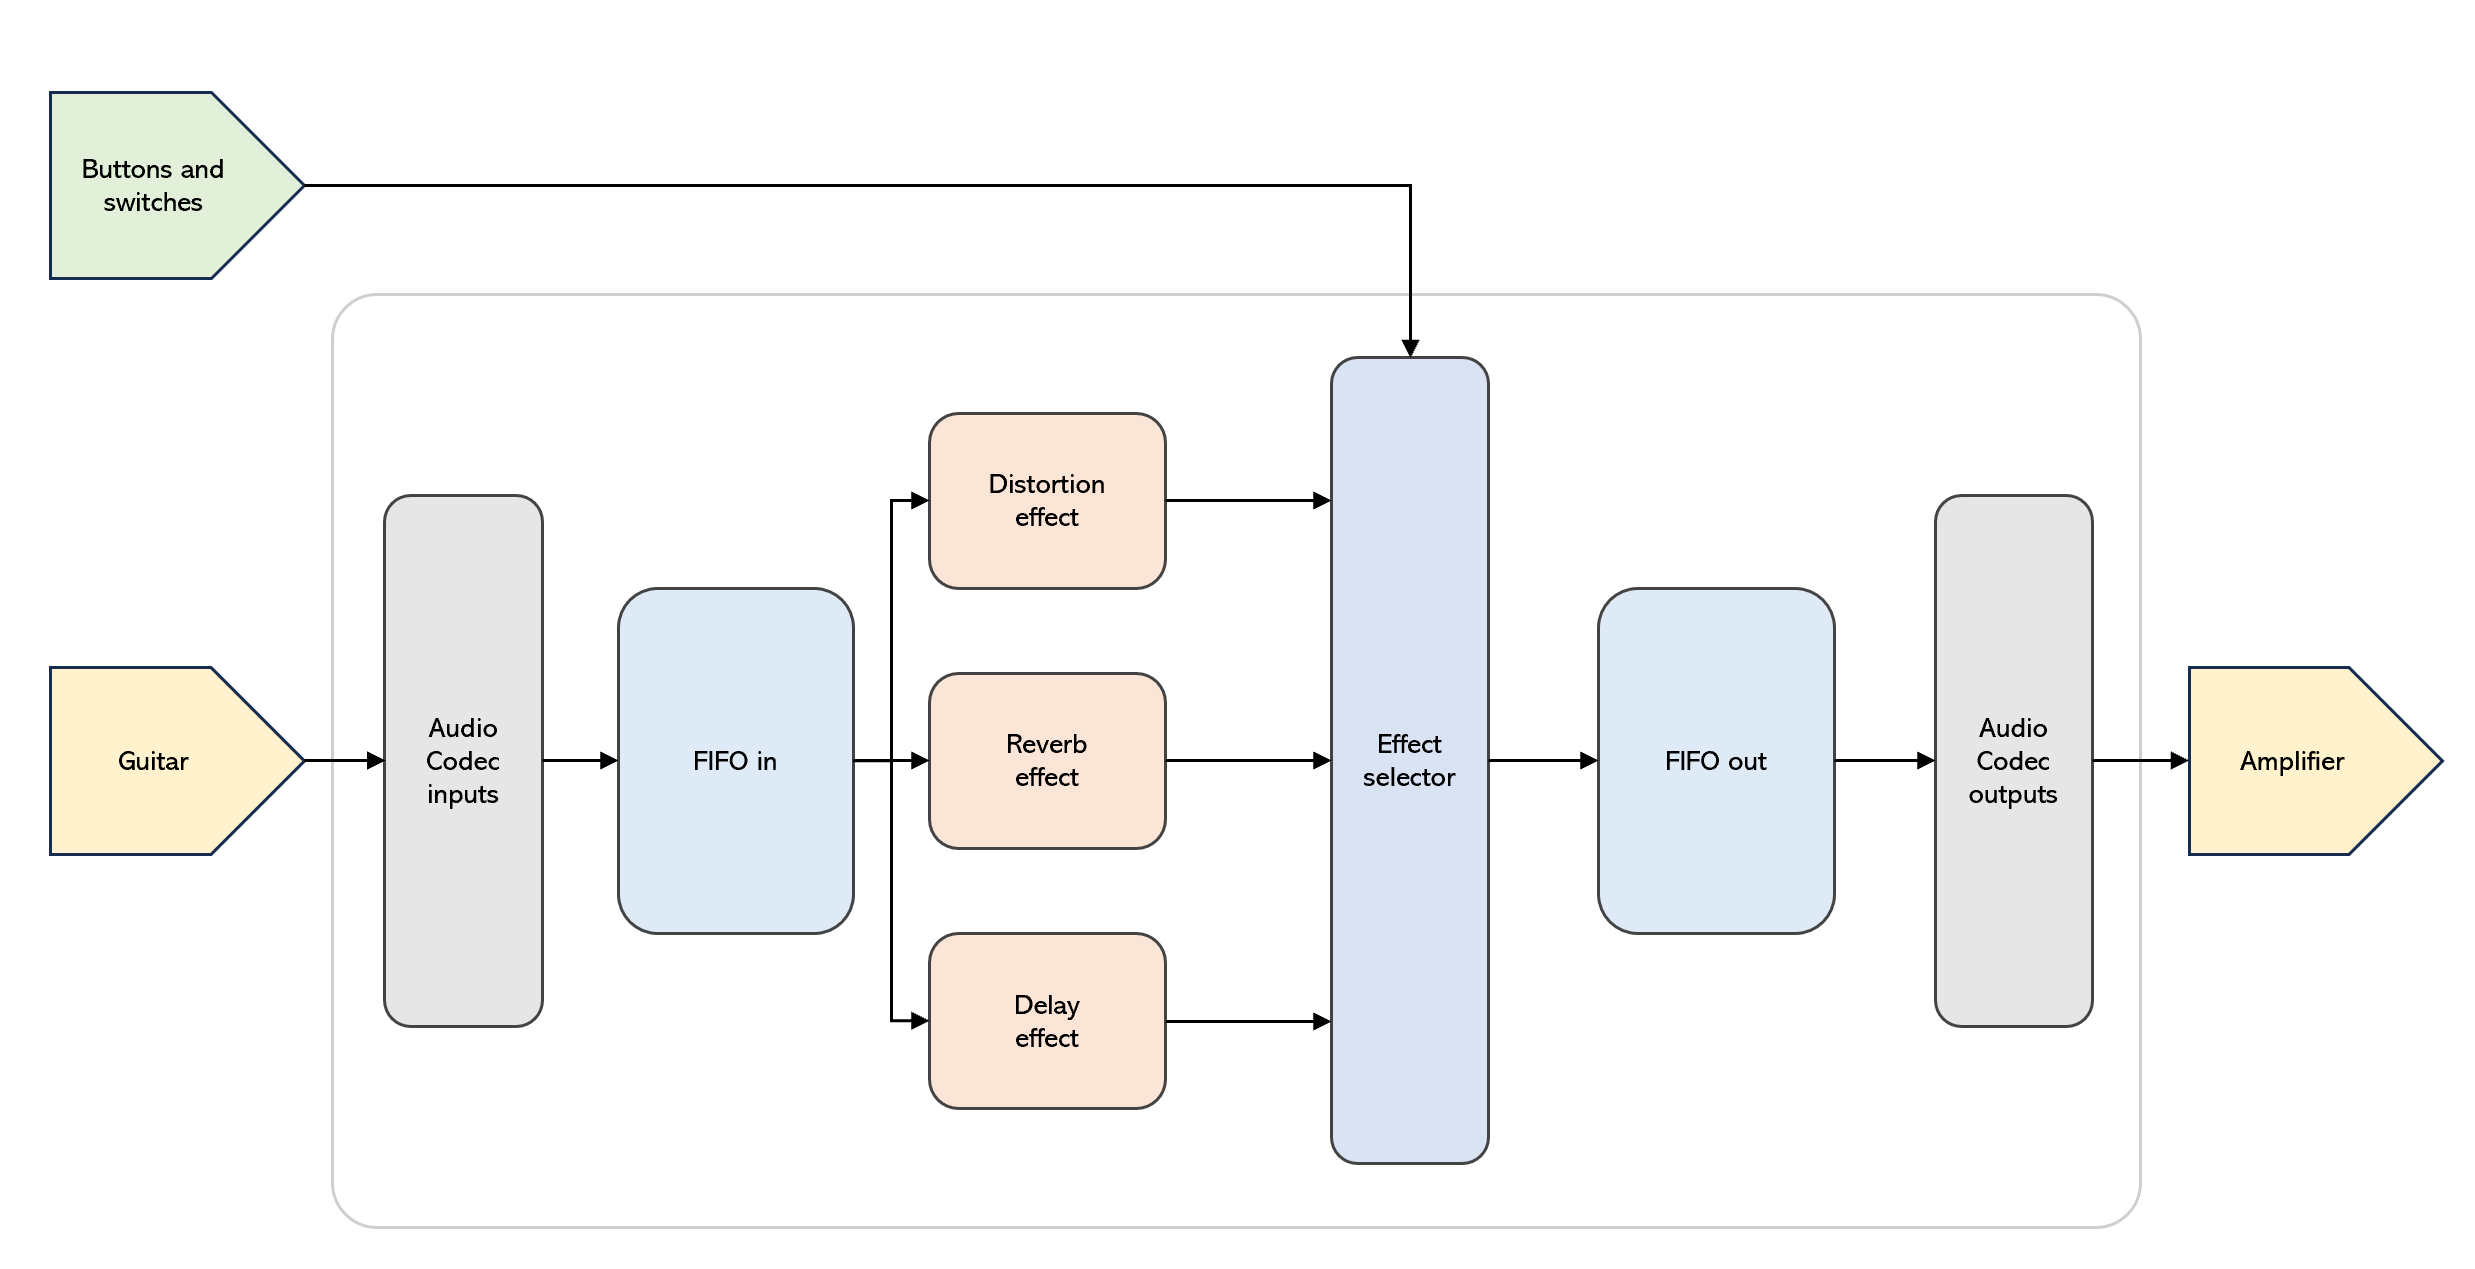
\includegraphics[width=1\linewidth]{progress-report/system-diagram.png}
    \caption{Simplified Diagram of Desired Audio Effects System}
    \label{fig:system-diagram}
\end{figure}